\documentclass[10pt]{article}
\usepackage[margin=1.7cm]{geometry}
\usepackage[T1]{fontenc}
\usepackage{lmodern}
\usepackage{microtype}
\usepackage{booktabs}
\usepackage{enumitem}
\usepackage{titlesec}
\usepackage{graphicx}
\usepackage{float}
\usepackage[hidelinks]{hyperref}

\titlespacing*{\section}{0pt}{7pt}{2pt}
\titleformat*{\section}{\normalsize\bfseries}
\setlist{nosep,leftmargin=1.2em,itemsep=1pt}
\setlength{\parskip}{3pt}
\setlength{\parindent}{0pt}
\setlength{\abovecaptionskip}{3pt}

\title{\vspace{-1.5cm}\large\textbf{XBRL Leaderboard: What Small Open-Weight Models Can Do on XBRL Tasks, and at What Cost}}
\author{\normalsize Dev Gaglani \quad Stavan Desai}
\date{}

\begin{document}
\maketitle
\vspace{-1.3cm}

\section{Research question and gap}
Banks and regulators often need models they can run in-house, which in practice means small open-weight models
(under about 10B parameters). Belcak et al.~[7] argue such models suit narrow, strictly formatted agent tasks, and name
the lack of task-specific benchmarks as a barrier. XBRL tagging is such a task. The group has XBRL benchmarks
(FinTagging~[1], XBRL-Agent~[2], FinAuditing~[3]) but no public page comparing models on them, and the Open FinLLM
Leaderboard~[4,5] has no XBRL tasks.

\textbf{Question:} \emph{On XBRL tasks, what can small open-weight models do on an ordinary laptop, where do they fail,
and what does each answer cost in time and memory?}

\section{Scope and evaluation}
\begin{itemize}
\item \textbf{Tasks:} concept linking (FinTagging public subset; 484 scored items after merging duplicates and
excluding conflicts, among 17{,}388 US-GAAP concepts) and financial calculation (XBRL-Agent, 1{,}000 formula questions).
FinAuditing comes later.
\item \textbf{Models:} seven instruction-tuned models from 1.5B to 8B: Qwen2.5 (1.5B, 3B, 7B), Llama-3.2-3B,
Llama-3.1-8B, Gemma-2-2B and Mistral-7B. All run locally through Ollama, 4-bit, greedy decoding, same inputs.
\item \textbf{Conditions (linking):} no tools; tag search over all concepts (100 candidates); search limited to
numeric concept types (a fixed list, not tuned on test items); and search limited to the item's \emph{given} type.
The given type always equals the correct concept's type, so this last condition is an \textbf{oracle diagnostic},
labelled as such and never ranked.
\item \textbf{Reported:} accuracy with 95\% confidence intervals, median latency per item, and peak memory, on two
machines kept separate: a Windows laptop (RTX~4050, 6\,GB) and an Apple M4 Mac (16\,GB).
\item \textbf{Scorer check:} we ran FinTagging's official evaluation code on our saved answers. It agrees item for
item for six of the seven models. For Llama-3.1-8B it fails to parse pretty-printed JSON and falls
back to the first candidate (75 correct by our scorer, 39 by the official one). We report ours and note
the official number.
\end{itemize}

\section{Results so far}
\begin{itemize}
\item \textbf{Linking:} without tools every model is below 2\%. With tag search (no oracle), the best is Qwen2.5-7B with
61 of 484 (12.6\%), and 71 (14.7\%) when the search is limited to numeric types. Even 1.5B to 3B models reach 8 to
12\%. The oracle type adds little on top (Qwen2.5-7B: 75, 15.5\%). The FinTagging paper reports 18.3\% for GPT-4o on its
full set.
\item \textbf{Why they fail:} retrieval is the larger problem. The correct concept is among the 100 candidates for only
134 of 484 items without a type filter (27.7\%) and 171 (35.3\%) with the oracle type. When it is there, the best
models pick it 42 to 47\% of the time and the smallest 25 to 32\%.
\item \textbf{Calculation (all seven models):} a formula lookup plus a calculator helps four models (Qwen2.5-7B from
65.7\% to 76.4\%; Llama-3.1-8B from 60.3\% to 73.2\%; Llama-3.2-3B and Gemma-2-2B) and hurts three that often write
an expression the calculator cannot evaluate (Qwen2.5-3B, Mistral-7B; Qwen2.5-1.5B from 66.9\% to 30.1\%).
\item \textbf{Cost:} on the 6\,GB laptop GPU, Qwen2.5-7B takes 4{,}535\,MiB and 1.6\,s per linking answer with tag
search; on the M4 Mac the same model takes 15.7\,s, mostly reading the 2{,}000-token prompt. Mac accuracy is within the
Windows confidence interval for every model and condition.
\end{itemize}
Every number on the page (Figure~1) is recomputed by a script from the saved answers and checked against the raw data.
\begin{figure}[t]
\centering
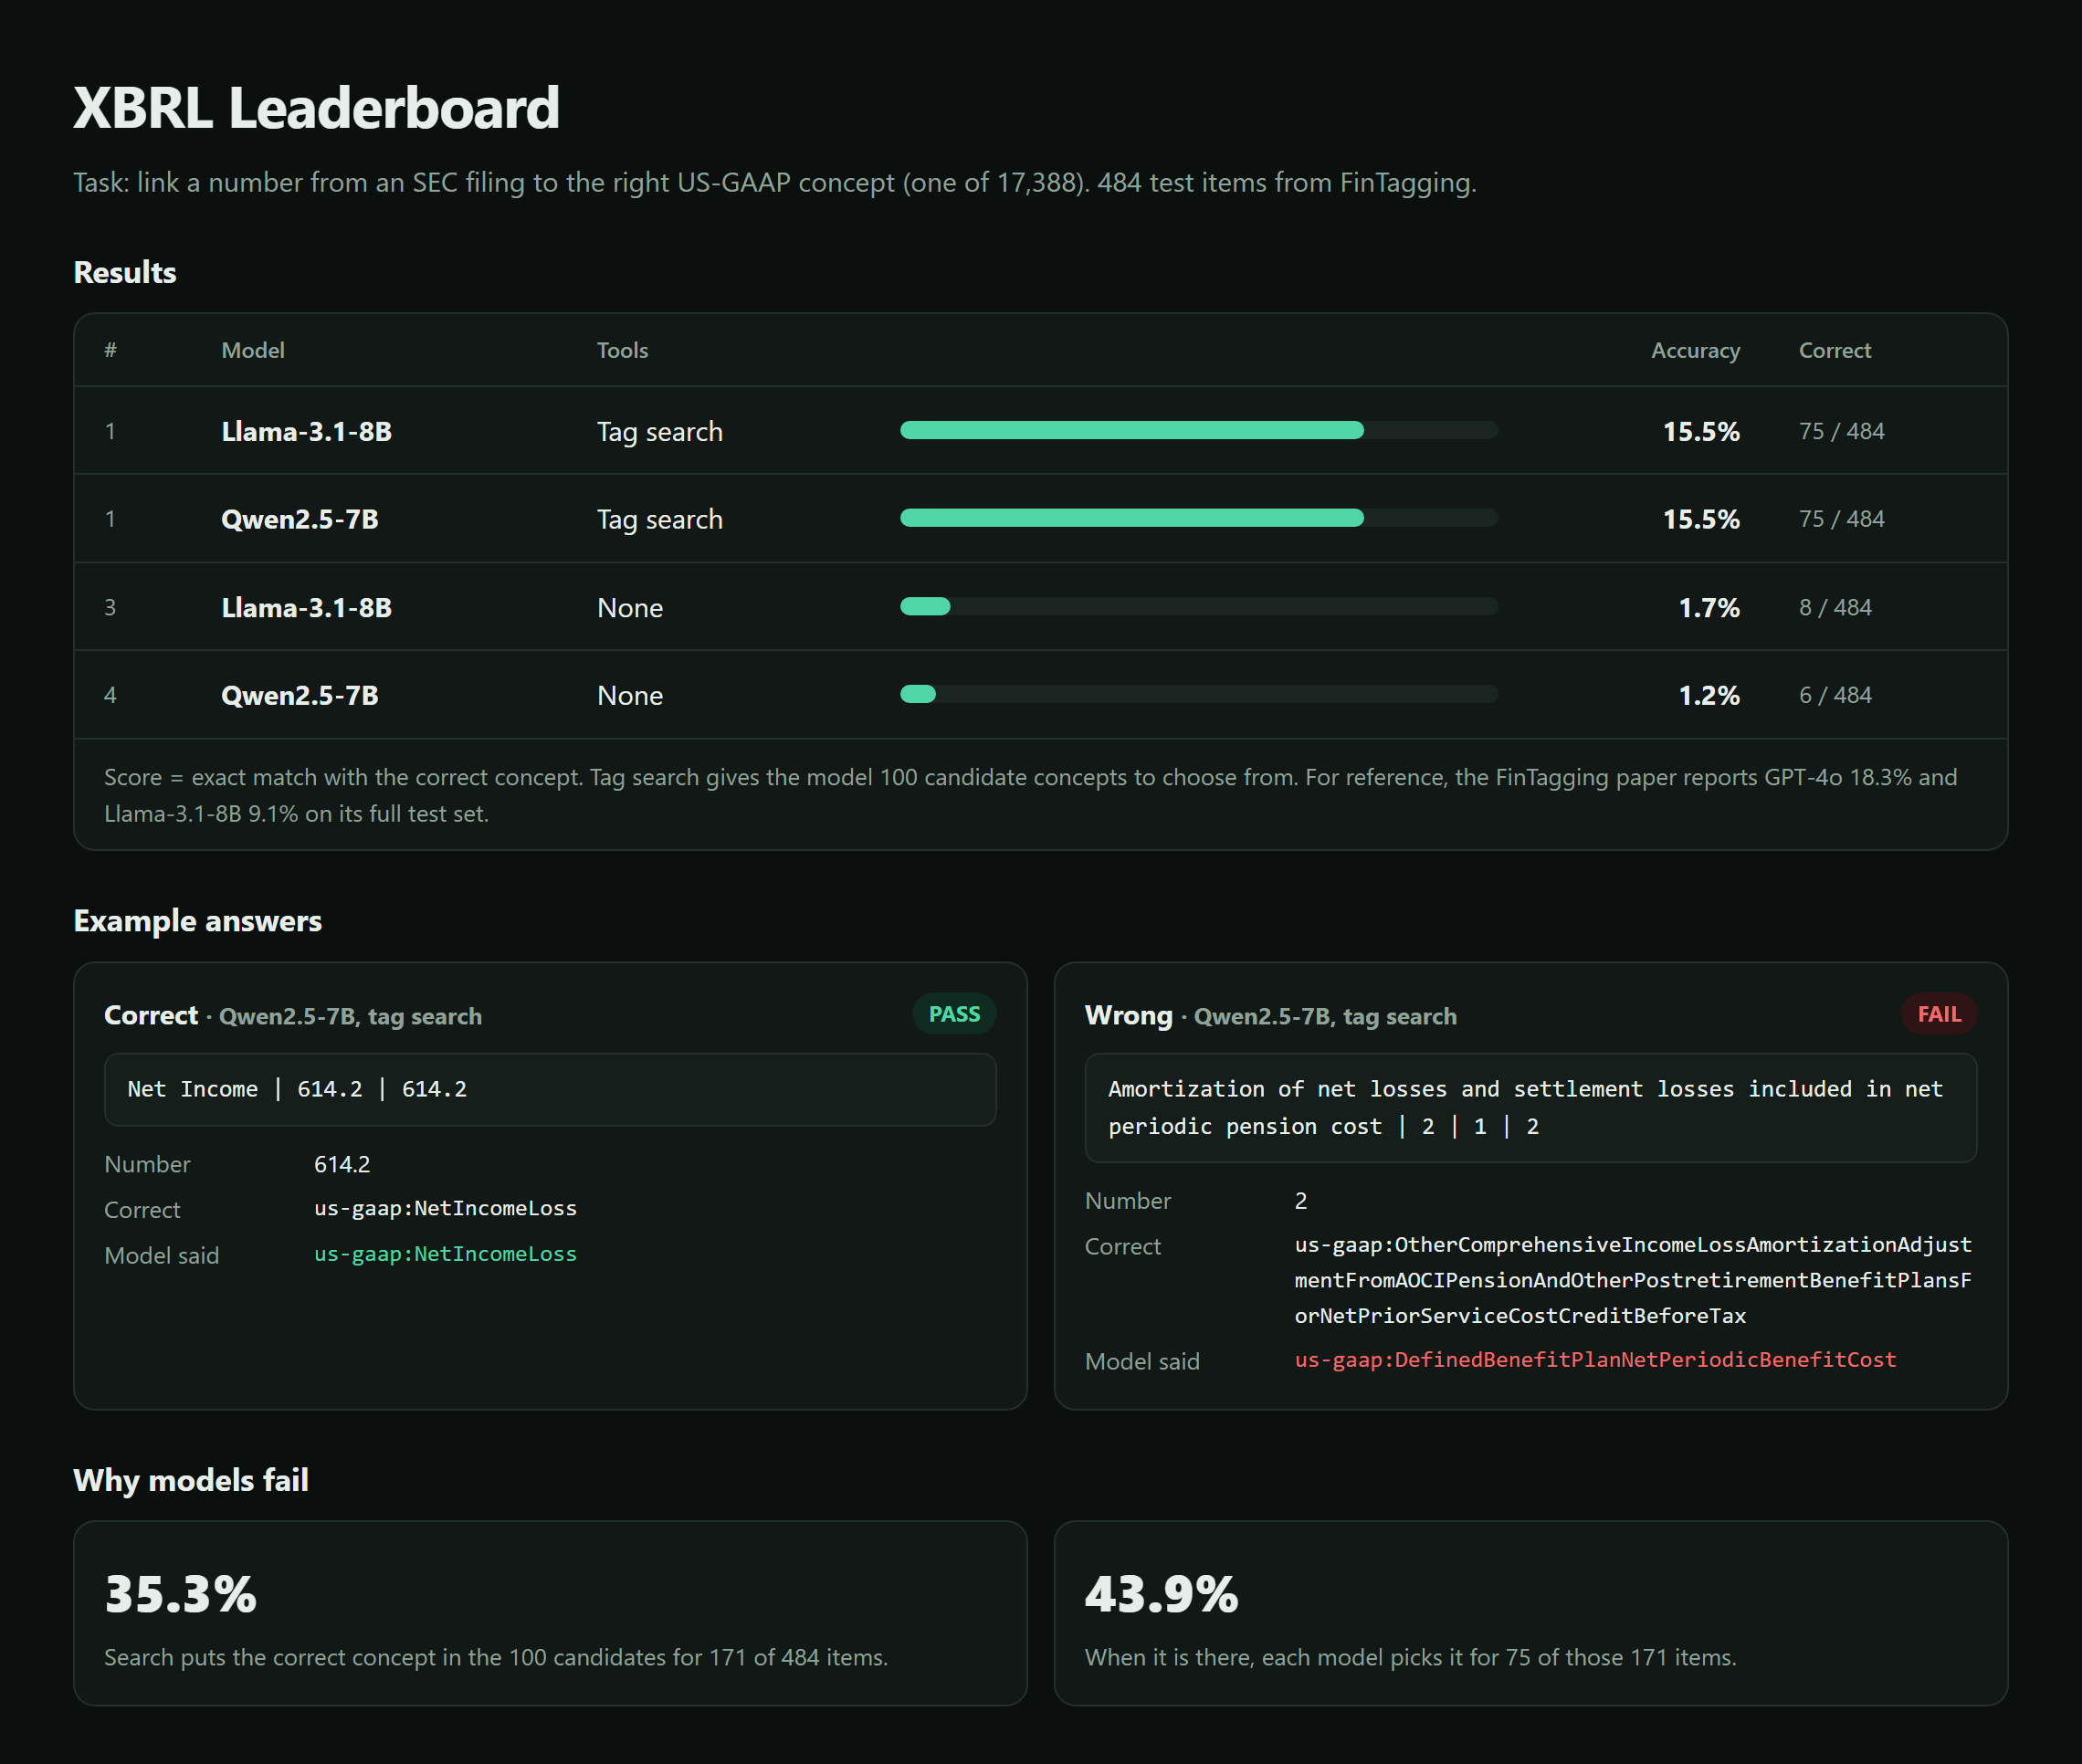
\includegraphics[width=0.46\textwidth]{demo_screenshot.png}
\caption{\footnotesize The page: accuracy for each model and condition, cost on each laptop, and why models fail.
A second tab shows the calculation task.}
\end{figure}

\section{What we reuse and what we add}
\begin{itemize}
\item \textbf{Reuse:} the group's datasets and metrics, FinTagging's official evaluation code (checked above), and the
Open FinLLM Leaderboard code.
\item \textbf{Add:} an XBRL page with models, conditions, accuracy, latency and memory. In the leaderboard code the task
columns are hard-coded, so our first change makes them configurable and adds a tools field.
\item \textbf{Reproducible:} code, saved answers, model digests and dataset commits are public on GitHub, under the MIT
licence for the code. The page is static and can be hosted on GitHub Pages.
\end{itemize}

\section{Next steps and roles}
{\centering\small
\begin{tabular}{p{2.3cm}p{10.4cm}p{2.4cm}}
\toprule
When & Work & Lead \\
\midrule
23--27 Nov & Share the page link; merge the Mac results; tag v0.1 & Dev \\
23--27 Nov & Calculation on the Mac; page updates; hosting & Stavan \\
30 Nov--4 Dec & Second XBRL task on the page (terminology or FinAuditing, as you prefer) & Both \\
7--18 Dec & Small Open FinLLM Leaderboard change (configurable tasks, tools field); short report & Both \\
\bottomrule
\end{tabular}\par}
\vspace{3pt}
Dev leads the evaluation; Stavan leads the page. We review results together.

\section{Where we need help}
\begin{itemize}
\item Is there a FinTagging task file for the group's evaluation suite that we should use instead of FinTagging's own
evaluation code? We found none in the public repositories.
\item Should the page live in our repository or under the group's organisation, and who reviews changes?
\item Which task should come second: XBRL-Agent terminology or FinAuditing?
\end{itemize}

\vspace{4pt}
{\footnotesize\textbf{References.}
[1] Y.~Wang et al. FinTagging. arXiv:2505.20650, 2025.
[2] S.~Han et al. XBRL Agent. ICAIF, 2024.
[3] Y.~Wang et al. FinAuditing. arXiv:2510.08886, 2025.
[4] S.~C.~Lin et al. Open FinLLM Leaderboard: Towards financial AI readiness. arXiv:2501.10963, 2025.
[5] S.~Lin et al. Evaluation and benchmarking suite for financial LLMs and agents. arXiv:2602.19073, 2026.
[6] Q.~Xie et al. FinBen. arXiv:2402.12659, 2024.
[7] P.~Belcak et al. Small language models are the future of agentic AI. arXiv:2506.02153, 2025.\par}
\end{document}
